\section{Рабочий проект}

\subsection{Модули программной системы}

\subsubsection{Модуль programm.py}

Модуль предоставляет основной графический интерфейс системы распознавания и управляет всеми процессами работы программы.

Класс - App.

Описание класса App:
Класс является центральным компонентом системы, управляющим всеми функциями распознавания. Базовый класс -- tk.Tk, стандартный класс библиотеки Tkinter. Интерфейсы -- главное меню с тремя режимами работы, виджеты для добавления пользователя и распознавания, система обработки видео с камеры.

Внутренние поля класса представлены в таблице~\ref{table:programm_fields}.

\renewcommand{\arraystretch}{0.8} % уменьшение расстояний до сетки таблицы
\begin{xltabular}{\textwidth}{|p{4.5cm}|>{\setlength{\baselineskip}{0.7\baselineskip}}p{4.5cm}|>{\setlength{\baselineskip}{0.7\baselineskip}}X|}
	\caption{Внутренние поля класса App\label{table:programm_fields}}\\
	\hline \centrow \setlength{\baselineskip}{0.7\baselineskip} Внутреннее поле & \centrow \setlength{\baselineskip}{0.7\baselineskip} Тип поля & \centrow Описание поля\\ \hline
	\endfirsthead
	\caption*{Продолжение таблицы \ref{table:programm_fields}}\\
	\hline \centrow \setlength{\baselineskip}{0.7\baselineskip} Внутреннее поле & \centrow \setlength{\baselineskip}{0.7\baselineskip} Тип поля & \centrow Описание поля\\ \hline
	\finishhead
	root & tk.Tk & Главное окно Tkinter \\
	\hline
	database & str & Путь к директории с файлами \\
	\hline
	fprints & str & Путь к директории отпечатков пальцев \\
	\hline
	embeddings\_path & str & Путь к директории векторных признаков \\
	\hline
	cards\_path & str & Путь к директории карт \\
	\hline
	faces\_path & str & Путь к директории лиц \\
	\hline
	embeddings & dict & Словарь векторных признаков пользователей \\
	\hline
	device & torch.device & Устройство для вычислений \\
	\hline
	detector & MTCNN & Детектор лиц \\
	\hline
	inception & InceptionResnetV1 & Модель векторных признаков лиц \\
	\hline
	fingerprints & Fingerprints & Объект для сравнения отпечатков \\
	\hline
	running & bool & Флаг, указывающий, работает ли приложение \\
	\hline
	current\_mode & str или None & Текущий режим приложения \\
	\hline
	current\_user & str или None & Текущий распознанный пользователь \\
	\hline
	video\_label & tk.Label или None & Метка для отображения видеопотока \\
	\hline
	cap & cv2.VideoCapture или None & Объект захвата видео \\
	\hline
	start\_time & float или None & Метка времени для обработки кадров \\
	\hline
	user\_name\_entry & ttk.Entry или None & Поле ввода имени пользователя \\
\end{xltabular}
\renewcommand{\arraystretch}{1.0} % восстановление сетки

Методы класса представлены в таблице~\ref{table:programm.py}.

\renewcommand{\arraystretch}{0.8} % уменьшение расстояний до сетки таблицы
\begin{xltabular}{\textwidth}{|>{\raggedright\arraybackslash}X|>{\raggedright\arraybackslash}X|>{\raggedright\arraybackslash\setlength{\baselineskip}{0.7\baselineskip}}X|>{\raggedright\arraybackslash\setlength{\baselineskip}{0.7\baselineskip}}X|}
\caption{Методы класса App\label{table:programm.py}}\\
\hline \centrow \setlength{\baselineskip}{0.7\baselineskip} Название метода & \centrow \setlength{\baselineskip}{0.7\baselineskip} Параметры метода & \centrow Возвращаемое значение & \centrow Описание метода \\ \hline
\endfirsthead
\caption*{Продолжение таблицы \ref{table:programm.py}}\\ 
\hline \centrow \setlength{\baselineskip}{0.7\baselineskip} Название метода & \centrow \setlength{\baselineskip}{0.7\baselineskip} Параметры метода & \centrow Возвращаемое значение & \centrow Описание метода \\ \hline
\finishhead
\_\_init\_\_ & root, device, detector, inception, embeddings & Отсутствует & Инициализирует главное окно приложения \\ 
\hline
show\_main\_menu & Отсутствуют & Отсутствует & Отображает главное меню \\ 
\hline
start\_add\_user \_mode & Отсутствуют & Отсутствует & Переключает в режим добавления пользователя \\ 
\hline
start\_recognition \_mode & Отсутствуют & Отсутствует & Переключает в режим распознавания \\ 
\hline
capture\_user\_face & Отсутствуют & Отсутствует & Захватывает изображения лица пользователя \\ 
\hline
add\_fingerprint & Отсутствуют & Отсутствует & Добавляет отпечаток пальца \\ 
\hline
create\_user\_card & Отсутствуют & Отсутствует & Создает QR-код карты пользователя \\ 
\hline
show\_qr\_code & image\_path: str — путь к изображению QR-кода & Отсутствует & Отображает QR-код в отдельном окне \\ 
\hline
card\_reader & Отсутствуют & Отсутствует & Обрабатывает видеопоток для чтения карт \\ 
\hline
read\_card & frame: np.ndarray — кадр видео & tuple[bool, str] — статус выполнения и декодированные данные & Распознает QR-код на кадре \\ 
\hline
process\_detected \_card & card: str — декодированные данные QR-кода & Отсутствует & Обрабатывает обнаруженную карту \\ 
\hline
verify\_user & Отсутствуют & Отсутствует & Проверяет пользователя по лицу и отпечатку \\ 
\hline
clear\_window & Отсутствуют & Отсутствует & Очищает окно приложения \\ 
\hline
on\_close & Отсутствуют & Отсутствует & Завершает работу приложения \\ 
\hline
\end{xltabular}
\renewcommand{\arraystretch}{1.0} % восстановление сетки

Класс - LoadingScreen.

Описание класса LoadingScreen:
Отображает экран загрузки во время инициализации моделей. Базовый класс -- tk.Tk, стандартный класс библиотеки Tkinter.

Внутренние поля класса представлены в таблице~\ref{table:LoadingScreen}.

\renewcommand{\arraystretch}{0.8} % уменьшение расстояний до сетки таблицы
\begin{xltabular}{\textwidth}{|p{4.5cm}|>{\setlength{\baselineskip}{0.7\baselineskip}}p{4.5cm}|>{\setlength{\baselineskip}{0.7\baselineskip}}X|}
	\caption{Внутренние поля класса LoadingScreen\label{table:LoadingScreen}}\\
	\hline \centrow \setlength{\baselineskip}{0.7\baselineskip} Внутреннее поле & \centrow \setlength{\baselineskip}{0.7\baselineskip} Тип поля & \centrow Описание поля\\ \hline
	\endfirsthead
	\caption*{Продолжение таблицы \ref{table:LoadingScreen}}\\
	\hline \centrow \setlength{\baselineskip}{0.7\baselineskip} Внутреннее поле & \centrow \setlength{\baselineskip}{0.7\baselineskip} Тип поля & \centrow Описание поля\\ \hline
	\finishhead
	root & tk.Tk & Главное окно Tkinter \\
	\hline
	top & tk.Toplevel & Окно экрана загрузки \\
	\hline
	label & tk.Label & Метка с сообщением о загрузке \\
	\hline
\end{xltabular}
\renewcommand{\arraystretch}{1.0} % восстановление сетки

Методы класса представлены в таблице~\ref{table:LoadingScreen.py}.

\renewcommand{\arraystretch}{0.8} % уменьшение расстояний до сетки таблицы
\begin{xltabular}{\textwidth}{|>{\raggedright\arraybackslash}X|>{\raggedright\arraybackslash}X|>{\raggedright\arraybackslash\setlength{\baselineskip}{0.7\baselineskip}}X|>{\raggedright\arraybackslash\setlength{\baselineskip}{0.7\baselineskip}}X|}
	\caption{Методы класса LoadingScreen\label{table:LoadingScreen.py}}\\
	\hline \centrow \setlength{\baselineskip}{0.7\baselineskip} Название метода & \centrow \setlength{\baselineskip}{0.7\baselineskip} Параметры метода & \centrow Возвращаемое значение & \centrow Описание метода \\ \hline
	\endfirsthead
	\caption*{Продолжение таблицы \ref{table:LoadingScreen.py}}\\ 	
	\hline \centrow \setlength{\baselineskip}{0.7\baselineskip} Название метода & \centrow \setlength{\baselineskip}{0.7\baselineskip} Параметры метода & \centrow Возвращаемое значение & \centrow Описание метода \\ \hline
	\finishhead
	destroy & Отсутствуют & Отсутствует & Закрывает экран загрузки \\ 
	\hline
\end{xltabular}
\renewcommand{\arraystretch}{1.0} % восстановление сетки

\subsubsection{Модуль save\_face.py}

Модуль содержит функцию для захвата изображений лиц.

Методы модуля представлены в таблице~\ref{table:save_face.py}.

\renewcommand{\arraystretch}{0.8} % уменьшение расстояний до сетки таблицы
\begin{xltabular}{\textwidth}{|>{\raggedright\arraybackslash}X|>{\raggedright\arraybackslash}X|>{\raggedright\arraybackslash\setlength{\baselineskip}{0.7\baselineskip}}X|>{\raggedright\arraybackslash\setlength{\baselineskip}{0.7\baselineskip}}X|}
	\caption{Методы модуля save\_face.py\label{table:save_face.py}}\\
	\hline \centrow \setlength{\baselineskip}{0.7\baselineskip} Название метода & \centrow \setlength{\baselineskip}{0.7\baselineskip} Параметры метода & \centrow Возвращаемое значение & \centrow Описание метода \\ \hline
	\endfirsthead
	\caption*{Продолжение таблицы \ref{table:save_face.py}}\\ 
	\hline \centrow \setlength{\baselineskip}{0.7\baselineskip} Название метода & \centrow \setlength{\baselineskip}{0.7\baselineskip} Параметры метода & \centrow Возвращаемое значение & \centrow Описание метода \\ \hline
	\finishhead
	capture\_faces & username: str — имя пользователя для организации сохранённых изображений лица & tuple(bool, int) — статус выполнения и количество захваченных изображений & Захватывает и сохраняет изображения лица \\ \hline
\end{xltabular}
\renewcommand{\arraystretch}{1.0} % восстановление сетки

\subsubsection{Модуль embedding\_create.py}

Модуль содержит функции для работы с векторными представлениями лиц.

Класс – FaceEmbedder.

Описание класса FaceEmbedder:
Генерирует векторные признаки лиц с использованием предобученных моделей MTCNN (детекция) и InceptionResnetV1 (кодирование). Базовый класс -- отсутствует. Интерфейсы -- отсутствуют.

Внутренние поля класса представлены в таблице~\ref{table:FaceEmbedder1}.

\renewcommand{\arraystretch}{0.8} % уменьшение расстояний до сетки таблицы
\begin{xltabular}{\textwidth}{|p{4.5cm}|>{\setlength{\baselineskip}{0.7\baselineskip}}p{4.5cm}|>{\setlength{\baselineskip}{0.7\baselineskip}}X|}
	\caption{Внутренние поля класса FaceEmbedder\label{table:FaceEmbedder1}}\\
	\hline \centrow \setlength{\baselineskip}{0.7\baselineskip} Внутреннее поле & \centrow \setlength{\baselineskip}{0.7\baselineskip} Тип поля & \centrow Описание поля\\ \hline
	\endfirsthead
	\caption*{Продолжение таблицы \ref{table:FaceEmbedder1}}\\
	\hline \centrow \setlength{\baselineskip}{0.7\baselineskip} Внутреннее поле & \centrow \setlength{\baselineskip}{0.7\baselineskip} Тип поля & \centrow Описание поля\\ \hline
	\finishhead
	
	device & torch.device & Устройство для выполнения вычислений (CPU/GPU)\\
	\hline 
	mtcnn & facenet\_pytorch. MTCNN & Модель для обнаружения лиц\\
	\hline 
	inception & facenet\_pytorch. InceptionResnetV1 & Модель извлечения признаков лица\\
	\hline
\end{xltabular}
\renewcommand{\arraystretch}{1.0} % восстановление сетки

Методы класса представлены в таблице~\ref{table:Embedder2}.

\renewcommand{\arraystretch}{0.8} % уменьшение расстояний до сетки таблицы
\begin{xltabular}{\textwidth}{|>{\raggedright\arraybackslash}X|>{\raggedright\arraybackslash}X|>{\raggedright\arraybackslash\setlength{\baselineskip}{0.7\baselineskip}}X|>{\raggedright\arraybackslash\setlength{\baselineskip}{0.7\baselineskip}}X|}
	\caption{Методы класса FaceEmbedder\label{table:Embedder2}}\\
	\hline \centrow \setlength{\baselineskip}{0.7\baselineskip} Название метода & \centrow \setlength{\baselineskip}{0.7\baselineskip} Параметры метода & \centrow Возвращаемое значение & \centrow Описание метода \\ \hline
	\endfirsthead
	\caption*{Продолжение таблицы \ref{table:Embedder2}}\\ 
	\hline \centrow \setlength{\baselineskip}{0.7\baselineskip} Название метода & \centrow \setlength{\baselineskip}{0.7\baselineskip} Параметры метода & \centrow Возвращаемое значение & \centrow Описание метода \\ \hline
	\finishhead
	\_\_init\_\_ & Отсутствуют & Отсутствуют & Инициализирует модели для извлечения признаков лица \\ \hline
	get\_embedding & img\_path: str — путь к изображению лица & np.ndarray — признаки лица, None — если обнаружение лица не удалось & Извлекает признаки лица лица из изображения \\ \hline
\end{xltabular}
\renewcommand{\arraystretch}{1.0} % восстановление сетки

Методы модуля представлены в таблице~\ref{table:Embedder3}.

\renewcommand{\arraystretch}{0.8} % уменьшение расстояний до сетки таблицы
\begin{xltabular}{\textwidth}{|>{\raggedright\arraybackslash}X|>{\raggedright\arraybackslash}X|>{\raggedright\arraybackslash\setlength{\baselineskip}{0.7\baselineskip}}X|>{\raggedright\arraybackslash\setlength{\baselineskip}{0.7\baselineskip}}X|}
	\caption{Методы модуля embedding\_create.py\label{table:Embedder3}}\\
	\hline \centrow \setlength{\baselineskip}{0.7\baselineskip} Название метода & \centrow \setlength{\baselineskip}{0.7\baselineskip} Параметры метода & \centrow Возвращаемое значение & \centrow Описание метода \\ \hline
	\endfirsthead
	\caption*{Продолжение таблицы \ref{table:Embedder3}}\\ 
	\hline \centrow \setlength{\baselineskip}{0.7\baselineskip} Название метода & \centrow \setlength{\baselineskip}{0.7\baselineskip} Параметры метода & \centrow Возвращаемое значение & \centrow Описание метода \\ \hline
	\finishhead
	\parbox[t]{\linewidth} {update\_user \_embedding} & username: str - имя пользователя & bool – статус выполнения & Вычисляет для указанного пользователя усредненное векторное представление лица по всем его изображениям и сохраняет в .npy-файл. \\ \hline
	get\_embeddings & Отсутствуют & dict[str, np.ndarray] — словарь, сопоставляющий имена пользователей их признакам лица. & Загружает все сохраненные векторные представления \\ \hline
\end{xltabular}
\renewcommand{\arraystretch}{1.0} % восстановление сетки

\subsubsection{Модуль func.py}

Модуль содержит вспомогательные функции для обнаружения лиц, генерации векторных представлений и распознавания.

Методы модуля представлены в таблице~\ref{table:func.py}.

\renewcommand{\arraystretch}{0.8} % уменьшение расстояний до сетки таблицы
\begin{xltabular}{\textwidth}{|>{\raggedright\arraybackslash}X|>{\raggedright\arraybackslash}X|>{\raggedright\arraybackslash\setlength{\baselineskip}{0.7\baselineskip}}X|>{\raggedright\arraybackslash\setlength{\baselineskip}{0.7\baselineskip}}X|}
	\caption{Методы модуля func.py\label{table:func.py}}\\
	\hline \centrow \setlength{\baselineskip}{0.7\baselineskip} Название метода & \centrow \setlength{\baselineskip}{0.7\baselineskip} Параметры метода & \centrow Возвращаемое значение & \centrow Описание метода \\ \hline
	\endfirsthead
	\caption*{Продолжение таблицы \ref{table:func.py}}\\ 
	\hline \centrow \setlength{\baselineskip}{0.7\baselineskip} Название метода & \centrow \setlength{\baselineskip}{0.7\baselineskip} Параметры метода & \centrow Возвращаемое значение & \centrow Описание метода \\ \hline
	\finishhead
	load\_models & Отсутствуют & tuple(torch.device, InceptionResnet, MTCNN) — устройство, модель признаков лица и детектор  & Загружает модели MTCNN и InceptionResnetV1 для обнаружения лиц и генерации эмбеддингов \\ 
	\hline
	camera\_connect & index: int — индекс камеры & cv2.VideoCapture — объект камеры & Пытается подключиться к камере по указанному индексу \\ 
	\hline
	detect\_faces & img: np.ndarray — входное изображение, embeddings: dict — словарь признаков пользователей, detector: MTCNN — детектор лиц, device: torch.device — устройство для вычислений, inception: InceptionResnetV1 — модель признаков & list[dict] — список обнаруженных лиц с их координатами, уверенностью, именем и оценкой схожести & Обнаруживает лица на изображении и распознаёт их \\ 
	\hline
	load\_embeddings & path: str — путь к директории с файлами признаков & dict[str, np.ndarray] — словарь, сопоставляющий имена пользователей признакам & Загружает все файлы признаков (.npy) из указанной директории \\ 
	\hline
	get\_embedding & face\_img: np.ndarray — изображение лица, device: torch.device — устройство для вычислений, inception: InceptionResnetV1 — модель признаков & np.ndarray или None — признаки лица или None при некорректном входе & Генерирует векторное представление для указанного изображения лица \\ 
	\hline
	recognize\_face & face: np.ndarray — изображение лица, embeddings: dict — словарь признаков пользователей, device: torch.device — устройство для вычислений, inception: InceptionResnetV1 — модель признаков & tuple(str, float) — имя пользователя и оценка схожести & Распознаёт лицо, сравнивая его признаки с сохранёнными \\ 
	\hline
	cosine\_similarity & vec: np.ndarray — тестовый вектор признаков, ref\_vecs: np.ndarray — опорный вектор признаков & np.ndarray или float — оценка сходства & Вычисляет косинусное сходство между тестовым и опорным вектором \\
	\hline
\end{xltabular}
\renewcommand{\arraystretch}{1.0} % восстановление сетки

\subsubsection{Модуль fp.py}

Модуль предназначен для сравнения отпечатков пальцев с использованием сиамской сети.

Класс – Fingerprints.

Описание класса Fingerprints:
Сравнивает изображения отпечатков пальцев с использованием предобученной сиамской сети. Базовый класс -- отсутствует. Интерфейсы -- отсутствуют.

Внутренние поля класса представлены в таблице~\ref{table:Fingerprints}.

\renewcommand{\arraystretch}{0.8} % уменьшение расстояний до сетки таблицы
\begin{xltabular}{\textwidth}{|p{4.5cm}|>{\setlength{\baselineskip}{0.7\baselineskip}}p{4.5cm}|>{\setlength{\baselineskip}{0.7\baselineskip}}X|}
	\caption{Внутренние поля класса Fingerprints\label{table:Fingerprints}}\\
	\hline \centrow \setlength{\baselineskip}{0.7\baselineskip} Внутреннее поле & \centrow \setlength{\baselineskip}{0.7\baselineskip} Тип поля & \centrow Описание поля\\ \hline
	\endfirsthead
	\caption*{Продолжение таблицы \ref{table:Fingerprints}}\\
	\hline \centrow \setlength{\baselineskip}{0.7\baselineskip} Внутреннее поле & \centrow \setlength{\baselineskip}{0.7\baselineskip} Тип поля & \centrow Описание поля\\ \hline
	\finishhead
	
	transform & torchvision.transforms. Compose & Трансформации для предобработки изображений\\
	\hline 
	device & torch.device & Устройство для вычислений\\
	\hline 
	model & SiameseNetwork & Предобученная модель сиамской сети\\
	\hline 
	model\_path & str & Путь к сохранённым весам модели\\
	\hline 
\end{xltabular}
\renewcommand{\arraystretch}{1.0} % восстановление сетки

Методы класса представлены в таблице~\ref{table:Fingerprints2}.

\renewcommand{\arraystretch}{0.8} % уменьшение расстояний до сетки таблицы
\begin{xltabular}{\textwidth}{|>{\raggedright\arraybackslash}X|>{\raggedright\arraybackslash}X|>{\raggedright\arraybackslash\setlength{\baselineskip}{0.7\baselineskip}}X|>{\raggedright\arraybackslash\setlength{\baselineskip}{0.7\baselineskip}}X|}
	\caption{Методы класса Fingerprints\label{table:Fingerprints2}}\\
	\hline \centrow \setlength{\baselineskip}{0.7\baselineskip} Название метода & \centrow \setlength{\baselineskip}{0.7\baselineskip} Параметры метода & \centrow Возвращаемое значение & \centrow Описание метода \\ \hline
	\endfirsthead
	\caption*{Продолжение таблицы \ref{table:Fingerprints2}}\\ 
	\hline \centrow \setlength{\baselineskip}{0.7\baselineskip} Название метода & \centrow \setlength{\baselineskip}{0.7\baselineskip} Параметры метода & \centrow Возвращаемое значение & \centrow Описание метода \\ \hline
	\finishhead
	\_\_init\_\_ & Отсутствуют & Отсутствует & Инициализирует модель для сравнения отпечатков \\ \hline
	compare\_images \_cosine & img\_path1: str — путь к первому изображению отпечатка, img\_path2: str — путь ко второму изображению отпечатка & float — оценка косинусного сходства & Сравнивает два отпечатка по косинусной близости \\ \hline
\end{xltabular}
\renewcommand{\arraystretch}{1.0} % восстановление сетки


\subsubsection{Модуль model.py}

Модуль определяет модели нейронных сетей для распознавания отпечатков пальцев -- FingerprintEncoder и SiameseNetwork.

Класс – FingerprintEncoder.

Описание класса FingerprintEncoder:
Кодирует изображения отпечатков пальцев в векторы признаков с использованием модели ResNet18. Базовый класс -- torch.nn.Module. Интерфейсы -- отсутствуют.

Внутренние поля класса представлены в таблице~\ref{table:FingerprintEncoder}.

\renewcommand{\arraystretch}{0.8} % уменьшение расстояний до сетки таблицы
\begin{xltabular}{\textwidth}{|p{4.5cm}|>{\setlength{\baselineskip}{0.7\baselineskip}}p{4.5cm}|>{\setlength{\baselineskip}{0.7\baselineskip}}X|}
	\caption{Внутренние поля класса FingerprintEncoder\label{table:FingerprintEncoder}}\\
	\hline \centrow \setlength{\baselineskip}{0.7\baselineskip} Внутреннее поле & \centrow \setlength{\baselineskip}{0.7\baselineskip} Тип поля & \centrow Описание поля\\ \hline
	\endfirsthead
	\caption*{Продолжение таблицы \ref{table:FingerprintEncoder}}\\
	\hline \centrow \setlength{\baselineskip}{0.7\baselineskip} Внутреннее поле & \centrow \setlength{\baselineskip}{0.7\baselineskip} Тип поля & \centrow Описание поля\\ \hline
	\finishhead
	
	encoder & \parbox[t]{\linewidth} {torchvision.models. resnet.ResNet} & Предобученная модель ResNet18 с заменённым полносвязным слоем на слой идентичности \\
\end{xltabular}
\renewcommand{\arraystretch}{1.0} % восстановление сетки

Методы класса представлены в таблице~\ref{table:model}.

\renewcommand{\arraystretch}{0.8} % уменьшение расстояний до сетки таблицы
\begin{xltabular}{\textwidth}{|>{\raggedright\arraybackslash}X|>{\raggedright\arraybackslash}X|>{\raggedright\arraybackslash\setlength{\baselineskip}{0.7\baselineskip}}X|>{\raggedright\arraybackslash\setlength{\baselineskip}{0.7\baselineskip}}X|}
	\caption{Методы класса FingerprintEncoder\label{table:model}}\\
	\hline \centrow \setlength{\baselineskip}{0.7\baselineskip} Название метода & \centrow \setlength{\baselineskip}{0.7\baselineskip} Параметры метода & \centrow Возвращаемое значение & \centrow Описание метода \\ \hline
	\endfirsthead
	\caption*{Продолжение таблицы \ref{table:model}}\\ 	
	\hline \centrow \setlength{\baselineskip}{0.7\baselineskip} Название метода & \centrow \setlength{\baselineskip}{0.7\baselineskip} Параметры метода & \centrow Возвращаемое значение & \centrow Описание метода \\ \hline
	\finishhead
	forward & x: torch.Tensor — входной тензор изображения & torch.Tensor — вектор признаков & Обрабатывает входное изображение через кодировщик ResNet18 для получения вектора признаков \\ \hline
\end{xltabular}
\renewcommand{\arraystretch}{1.0} % восстановление сетки

Класс – SiameseNetwork.

Описание класса SiameseNetwork:
Реализует сиамскую сеть для сравнения пар изображений отпечатков пальцев. Базовый класс -- torch.nn.Module. Интерфейсы -- отсутствуют. Константы -- отсутствуют.

Внутренние поля класса представлены в таблице~\ref{table:SiameseNetwork}.

\renewcommand{\arraystretch}{0.8} % уменьшение расстояний до сетки таблицы
\begin{xltabular}{\textwidth}{|p{4.5cm}|>{\setlength{\baselineskip}{0.7\baselineskip}}p{4.5cm}|>{\setlength{\baselineskip}{0.7\baselineskip}}X|}
	\caption{Внутренние поля класса SiameseNetwork\label{table:SiameseNetwork}}\\
	\hline \centrow \setlength{\baselineskip}{0.7\baselineskip} Внутреннее поле & \centrow \setlength{\baselineskip}{0.7\baselineskip} Тип поля & \centrow Описание поля\\ \hline
	\endfirsthead
	\caption*{Продолжение таблицы \ref{table:SiameseNetwork}}\\
	\hline \centrow \setlength{\baselineskip}{0.7\baselineskip} Внутреннее поле & \centrow \setlength{\baselineskip}{0.7\baselineskip} Тип поля & \centrow Описание поля\\ \hline
	\finishhead
	
	encoder & FingerprintEncoder & Экземпляр класса FingerprintEncoder для извлечения признаков \\ \hline
	fc & torch.nn.Sequential & Полносвязные слои для обработки разности векторов признаков и вывода оценки схожести \\ 
	\hline
\end{xltabular}
\renewcommand{\arraystretch}{1.0} % восстановление сетки

Методы класса представлены в таблице~\ref{table:model}.

\renewcommand{\arraystretch}{0.8} % уменьшение расстояний до сетки таблицы
\begin{xltabular}{\textwidth}{|>{\hsize=0.7\hsize\raggedright\arraybackslash}X|
		>{\hsize=1.0\hsize\setlength{\baselineskip}{0.7\baselineskip}}X|
		>{\hsize=1.0\hsize}X|
		>{\hsize=1.3\hsize}X|}
	\caption{Методы класса SiameseNetwork\label{table:model}}\\
	\hline 
	\centrow Название метода & 
	\centrow Параметры метода & 
	\centrow Возвращаемое значение &
	\centrow Описание метода \\ 
	\hline 
	\endfirsthead
	\caption*{Продолжение таблицы \ref{table:model}}\\ 
	\hline 
	\centrow Название метода & 
	\centrow Параметры метода & 
	\centrow Возвращаемое значение &
	\centrow Описание метода \\ 
	\hline 
	\finishhead
	forward & \parbox[t]{\linewidth} {img1: torch.Tensor — тензор первого изображения отпечатка, img2: torch.Tensor — тензор второго изображения отпечатка} & torch.Tensor — оценка схожести от 0 до 1 & Извлекает признаки из обоих изображений, вычисляет их абсолютную разность и пропускает через полносвязные слои для получения оценки схожести \\ 
	\hline
	forward\_once & \parbox[t]{\linewidth} {x: torch.Tensor — тензор одного изображения отпечатка} & torch.Tensor — вектор признаков & Извлекает признаки из одного изображения с помощью кодировщика \\ 
	\hline
\end{xltabular}
\renewcommand{\arraystretch}{1.0} % восстановление сетки

\subsubsection{Модуль dataset.py}

Модуль содержит функции для загрузки и подготовки пар изображений отпечатков пальцев для обучения сиамской сети.

Класс – FingerprintPairsDataset.

Описание класса FingerprintPairsDataset:
Создаёт пары изображений отпечатков пальцев (положительные и отрицательные пары) для обучения. Базовый класс -- torch.utils.data.Dataset. Интерфейсы -- отсутствуют.

Внутренние поля класса представлены в таблице~\ref{table:FingerprintPairsDataset}.

\renewcommand{\arraystretch}{0.8} % уменьшение расстояний до сетки таблицы
\begin{xltabular}{\textwidth}{|p{4.5cm}|>{\setlength{\baselineskip}{0.7\baselineskip}}p{4.5cm}|>{\setlength{\baselineskip}{0.7\baselineskip}}X|}
	\caption{Внутренние поля класса FingerprintPairsDataset\label{table:FingerprintPairsDataset}}\\
	\hline \centrow \setlength{\baselineskip}{0.7\baselineskip} Внутреннее поле & \centrow \setlength{\baselineskip}{0.7\baselineskip} Тип поля & \centrow Описание поля\\ \hline
	\endfirsthead
	\caption*{Продолжение таблицы \ref{table:FingerprintPairsDataset}}\\
	\hline \centrow \setlength{\baselineskip}{0.7\baselineskip} Внутреннее поле & \centrow \setlength{\baselineskip}{0.7\baselineskip} Тип поля & \centrow Описание поля\\ \hline
	\finishhead
	
	mine\_images & list[str] & Список путей к файлам изображений отпечатков пользователя\\
	\hline 
	others\_images & list[str] & Список путей к файлам изображений отпечатков других пользователей\\
	\hline 
	transform & torchvision.transforms. Compose & Трансформации для предобработки изображений\\
	\hline 
	positive\_pairs & list[tuple[str, str]] & Список пар изображений отпечатков одного пользователя\\
	\hline 
	negative\_pairs & list[tuple[str, str]] & Список пар, содержащих изображение пользователя и изображение другого человека\\
	\hline 
	pairs & list[tuple[str, str]] & Объединённый список положительных и отрицательных пар\\
	\hline 
	labels & list[int] & Метки (1 для положительных пар, 0 для отрицательных)\\
	\hline
\end{xltabular}
\renewcommand{\arraystretch}{1.0} % восстановление сетки

Методы класса представлены в таблице~\ref{table:FingerprintPairsDataset2}.

\renewcommand{\arraystretch}{0.8} % уменьшение расстояний до сетки таблицы
\begin{xltabular}{\textwidth}{|>{\raggedright\arraybackslash}X|>{\raggedright\arraybackslash}X|>{\raggedright\arraybackslash\setlength{\baselineskip}{0.7\baselineskip}}X|>{\raggedright\arraybackslash\setlength{\baselineskip}{0.7\baselineskip}}X|}
	\caption{Методы класса FingerprintPairsDataset\label{table:FingerprintPairsDataset2}}\\
	\hline \centrow \setlength{\baselineskip}{0.7\baselineskip} Название метода & \centrow \setlength{\baselineskip}{0.7\baselineskip} Параметры метода & \centrow Возвращаемое значение & \centrow Описание метода \\ \hline
	\endfirsthead
	\caption*{Продолжение таблицы \ref{table:FingerprintPairsDataset2}}\\ \hline \centrow \setlength{\baselineskip}{0.7\baselineskip} Название метода & \centrow \setlength{\baselineskip}{0.7\baselineskip} Параметры метода & \centrow Возвращаемое значение & \centrow Описание метода \\ \hline
	\finishhead
	\_\_len\_\_ & Отсутствуют & int — количество пар & Возвращает общее количество пар изображений \\ 
	\hline
	\_\_getitem\_\_ & idx: int — индекс пары & tuple(torch.Tensor, torch.Tensor, int) — два предобработанных тензора изображений и их метка & Загружает и предобрабатывает пару изображений по указанному индексу, возвращает изображения и их метку \\ \hline
\end{xltabular}
\renewcommand{\arraystretch}{1.0} % восстановление сетки

\subsubsection{Модуль train.py}

Модуль предназначен для обучения сиамской сети с целью распознавания отпечатков пальцев и предоставляет функцию для их сравнения.

Методы модуля представлены в таблице~\ref{table:train.py}.

\renewcommand{\arraystretch}{0.8} % уменьшение расстояний до сетки таблицы
\begin{xltabular}{\textwidth}{|>{\raggedright\arraybackslash}X|>{\raggedright\arraybackslash}X|>{\raggedright\arraybackslash\setlength{\baselineskip}{0.7\baselineskip}}X|>{\raggedright\arraybackslash\setlength{\baselineskip}{0.7\baselineskip}}X|}
	\caption{Методы модуля train.py\label{table:train.py}}\\
	\hline \centrow \setlength{\baselineskip}{0.7\baselineskip} Название метода & \centrow \setlength{\baselineskip}{0.7\baselineskip} Параметры метода & \centrow Возвращаемое значение & \centrow Описание метода \\ \hline
	\endfirsthead
	\caption*{Продолжение таблицы \ref{table:train.py}}\\ 
	\hline \centrow \setlength{\baselineskip}{0.7\baselineskip} Название метода & \centrow \setlength{\baselineskip}{0.7\baselineskip} Параметры метода & \centrow Возвращаемое значение & \centrow Описание метода \\ \hline
	\finishhead
	compare\_images & model: SiameseNetwork — обученная модель сиамской сети, img\_path1: str — путь к первому изображению отпечатка, img\_path2: str — путь ко второму изображению отпечатка & float — оценка схожести & Вычисляет оценку схожести между двумя изображениями отпечатков с использованием сиамской сети \\ 
	\hline
\end{xltabular}
\renewcommand{\arraystretch}{1.0} % восстановление сетки

\subsection{Модульное тестирование разработанного программного решения}

Модульный тест для модуля model.py представлен в таблице \ref{table:model_tests}.

\renewcommand{\arraystretch}{0.8} % уменьшение расстояний до сетки таблицы
\begin{xltabular}{\textwidth}{|>{\raggedright\arraybackslash}X|>{\raggedright\arraybackslash}X|>{\raggedright\arraybackslash\setlength{\baselineskip}{0.7\baselineskip}}X|>{\raggedright\arraybackslash\setlength{\baselineskip}{0.7\baselineskip}}X|}
	\caption{Модульное тестирование модуля model.py\label{table:model_tests}}\\
	\hline \centrow \setlength{\baselineskip}{0.7\baselineskip} Описание теста & \centrow \setlength{\baselineskip}{0.7\baselineskip} Входные данные & \centrow Ожидаемый результат \\ \hline
	\endfirsthead
	\caption*{Продолжение таблицы \ref{table:model_tests}}\\
	\hline \centrow \setlength{\baselineskip}{0.7\baselineskip} Описание теста & \centrow \setlength{\baselineskip}{0.7\baselineskip} Входные данные & \centrow Ожидаемый результат \\ \hline
	\finishhead
	Проверка вывода FingerprintEncoder & Тензор размера (1, 3, 500, 500) & Тензор размера (1, 512) \\ 
	\hline
	Проверка работы SiameseNetwork & Два одинаковых тензора (1, 3, 500, 500) & Значение в диапазоне [0, 1] \\ 
	\hline
	Проверка метода forward\_once & Тензор размера (1, 3, 500, 500) & Тензор размера (1, 512) \\ 
	\hline
\end{xltabular}
\renewcommand{\arraystretch}{1.0} % восстановление сетки



Модульный тест для модуля fp.py представлен в таблице \ref{table:fp_tests}.

\renewcommand{\arraystretch}{0.8} % уменьшение расстояний до сетки таблицы
\begin{xltabular}{\textwidth}{|>{\raggedright\arraybackslash}X|>{\raggedright\arraybackslash}X|>{\raggedright\arraybackslash\setlength{\baselineskip}{0.7\baselineskip}}X|>{\raggedright\arraybackslash\setlength{\baselineskip}{0.7\baselineskip}}X|}
	\caption{Модульное тестирование модуля fp.py\label{table:fp_tests}}\\
	\hline \centrow \setlength{\baselineskip}{0.7\baselineskip} Описание теста & \centrow \setlength{\baselineskip}{0.7\baselineskip} Входные данные & \centrow Ожидаемый результат \\ \hline
	\endfirsthead
	\caption*{Продолжение таблицы \ref{table:fp_tests}}\\
	\hline \centrow \setlength{\baselineskip}{0.7\baselineskip} Описание теста & \centrow \setlength{\baselineskip}{0.7\baselineskip} Входные данные & \centrow Ожидаемый результат \\ \hline
	\finishhead
	Инициализация класса Fingerprints & Имитация модели SiameseNetwork и torch.load & Успешное создание экземпляра \\ 
	\hline
	Сравнение двух изображений отпечатков & Пути к двум черно-белым изображениям (500x500) & Значение сходства в диапазоне [-1, 1] \\ 
	\hline
\end{xltabular}
\renewcommand{\arraystretch}{1.0} % восстановление сетки



Модульный тест для модуля func.py представлен в таблице \ref{table:func_tests}.

\renewcommand{\arraystretch}{0.8} % уменьшение расстояний до сетки таблицы
\begin{xltabular}{\textwidth}{|>{\raggedright\arraybackslash}X|>{\raggedright\arraybackslash}X|>{\raggedright\arraybackslash\setlength{\baselineskip}{0.7\baselineskip}}X|>{\raggedright\arraybackslash\setlength{\baselineskip}{0.7\baselineskip}}X|}
	\caption{Модульное тестирование модуля func.py\label{table:func_tests}}\\
	\hline \centrow \setlength{\baselineskip}{0.7\baselineskip} Описание теста & \centrow \setlength{\baselineskip}{0.7\baselineskip} Входные данные & \centrow Ожидаемый результат \\ \hline
	\endfirsthead
	\caption*{Продолжение таблицы \ref{table:func_tests}}\\
	\hline \centrow \setlength{\baselineskip}{0.7\baselineskip} Описание теста & \centrow \setlength{\baselineskip}{0.7\baselineskip} Входные данные & \centrow Ожидаемый результат \\ \hline
	\finishhead
	Загрузка эмбеддингов из папки & Папка с двумя .npy файлами эмбеддингов & Словарь с ключами 'user1', 'user2' и значениями-массивами \\ 
	\hline
	Получение эмбеддинга из изображения & Набор имитаций: модель, трансформации, изображение numpy & Эмбеддинг размером (512,) \\ 
	\hline
	Косинусное сходство между векторами & Два ортогональных вектора и два одинаковых & 0 (ортогональные), 1 (одинаковые) \\ 
	\hline
\end{xltabular}
\renewcommand{\arraystretch}{1.0} % восстановление сетки


Модульный тест для модуля dataset.py представлен в таблице \ref{table:dataset_tests}.

\renewcommand{\arraystretch}{0.8} % уменьшение расстояний до сетки таблицы
\begin{xltabular}{\textwidth}{|>{\raggedright\arraybackslash}X|>{\raggedright\arraybackslash}X|>{\raggedright\arraybackslash\setlength{\baselineskip}{0.7\baselineskip}}X|>{\raggedright\arraybackslash\setlength{\baselineskip}{0.7\baselineskip}}X|}
	\caption{Модульное тестирование модуля dataset.py\label{table:dataset_tests}}\\
	\hline \centrow \setlength{\baselineskip}{0.7\baselineskip} Описание теста & \centrow \setlength{\baselineskip}{0.7\baselineskip} Входные данные & \centrow Ожидаемый результат \\ \hline
	\endfirsthead
	\caption*{Продолжение таблицы \ref{table:dataset_tests}}\\
	\hline \centrow \setlength{\baselineskip}{0.7\baselineskip} Описание теста & \centrow \setlength{\baselineskip}{0.7\baselineskip} Входные данные & \centrow Ожидаемый результат \\ \hline
	\finishhead
	Проверка длины датасета & Папки с 3 изображениями нужного человека и 3 другого & Длина равна 6 \\ 
	\hline
	Проверка выдачи элемента датасета & Индекс 0 & Два изображения размера (500, 500) и метка 0 или 1 \\ 
	\hline
\end{xltabular}
\renewcommand{\arraystretch}{1.0} % восстановление сетки


Модульный тест для модуля embedding\_create.py представлен в таблице \ref{table:embedding_tests}.

\renewcommand{\arraystretch}{0.8} % уменьшение расстояний до сетки таблицы
\begin{xltabular}{\textwidth}{|>{\raggedright\arraybackslash}X|>{\raggedright\arraybackslash}X|>{\raggedright\arraybackslash\setlength{\baselineskip}{0.7\baselineskip}}X|>{\raggedright\arraybackslash\setlength{\baselineskip}{0.7\baselineskip}}X|}
	\caption{Модульное тестирование модуля embedding\_create.py\label{table:embedding_tests}}\\
	\hline \centrow \setlength{\baselineskip}{0.7\baselineskip} Описание теста & \centrow \setlength{\baselineskip}{0.7\baselineskip} Входные данные & \centrow Ожидаемый результат \\ \hline
	\endfirsthead
	\caption*{Продолжение таблицы \ref{table:embedding_tests}}\\
	\hline \centrow \setlength{\baselineskip}{0.7\baselineskip} Описание теста & \centrow \setlength{\baselineskip}{0.7\baselineskip} Входные данные & \centrow Ожидаемый результат \\ \hline
	\finishhead
	Получение эмбеддинга лица с имитациями моделей & Путь к изображению, имитация MTCNN, имитация модели InceptionResnetV1 & Эмбеддинг размером (512,) \\ 
	\hline
	Обновление эмбеддинга пользователя & Имя пользователя & True \\ 
	\hline
\end{xltabular}
\renewcommand{\arraystretch}{1.0} % восстановление сетки

\subsection{Системное тестирование разработанного программного решения}

На рисунке \ref{fig:main} представлено главное окно интеллектуальной системы.
\begin{figure}[H]
	\centering
	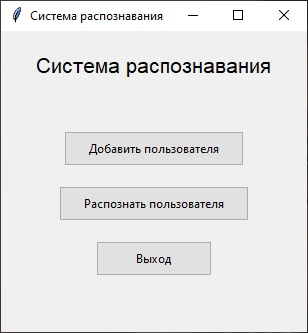
\includegraphics[width=0.5\linewidth]{images/main}
	\caption[]{Главное окно программы}
	\label{fig:main}
\end{figure}


На рисунке \ref{fig:add} представлено окно "Добавить пользователя".

\begin{figure}[H]
	\centering
	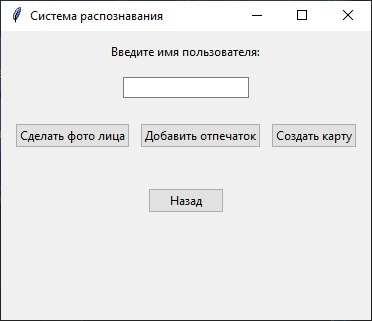
\includegraphics[width=0.7\linewidth]{images/add}
	\caption{Окно "Добавить пользователя"}
	\label{fig:add}
\end{figure}

На рисунке \ref{fig:errorname} представлено отображение ошибки при отстуствии введенного имени пользователя.

\begin{figure}[H]
	\centering
	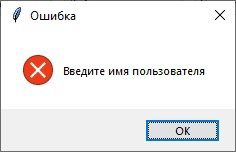
\includegraphics[width=0.6\linewidth]{images/errorname}
	\caption{Окно отображения ошибки "Введите имя пользователя"}
	\label{fig:errorname}
\end{figure}

На рисунке \ref{fig:embcreate} представлено отображение информации о сохранении признаков лица.

\begin{figure}[H]
	\centering
	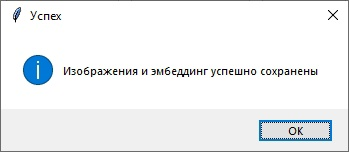
\includegraphics[width=0.7\linewidth]{images/embcreate}
	\caption{Окно отображения информации о сохранении признаков лица}
	\label{fig:embcreate}
\end{figure}

На рисунке \ref{fig:fp} представлено диалоговое окно выбора изображения с отпечатком пальца.

\begin{figure}[H]
	\centering
	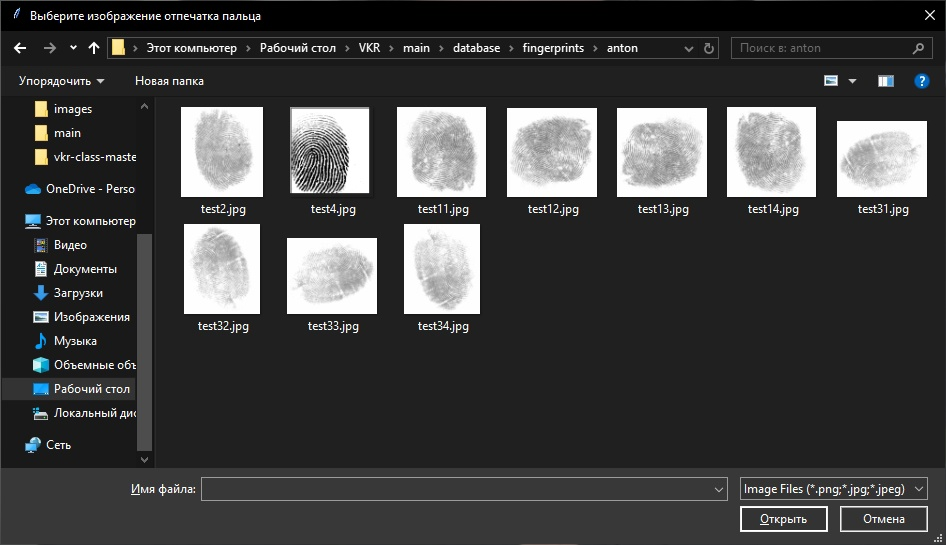
\includegraphics[width=0.9\linewidth]{images/fp}
	\caption{Диалоговое окно выбора изображения с отпечатком пальца}
	\label{fig:fp}
\end{figure}

На рисунке \ref{fig:fpinfo} представлено отображение информации о сохранении отпечатка пальца.

\begin{figure}[H]
	\centering
	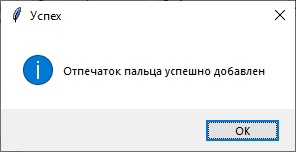
\includegraphics[width=0.6\linewidth]{images/fpinfo}
	\caption{Окно отображения информации о сохранении отпечатка пальца}
	\label{fig:fpinfo}
\end{figure}

На рисунке \ref{fig:qrinfo} представлено отображение информации о создании карты доступа.

\begin{figure}[H]
	\centering
	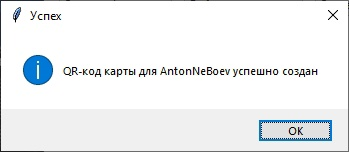
\includegraphics[width=0.65\linewidth]{images/qrinfo}
	\caption{Окно отображения информации о создании карты доступа}
	\label{fig:qrinfo}
\end{figure}

На рисунке \ref{fig:qr} представлено созданное для пользователя изображение карты доступа.
\begin{figure}[H]
	\centering
	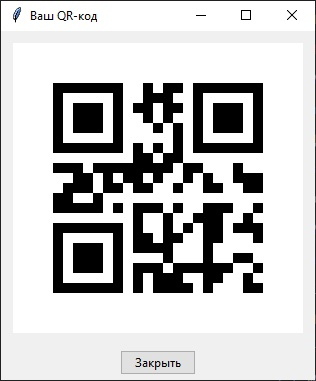
\includegraphics[width=0.5\linewidth]{images/qr}
	\caption{Окно отображения созданной карты}
	\label{fig:qr}
\end{figure}


На рисунке \ref{fig:define} представлено окно "Распознать пользователя".
\begin{figure}[H]
	\centering
	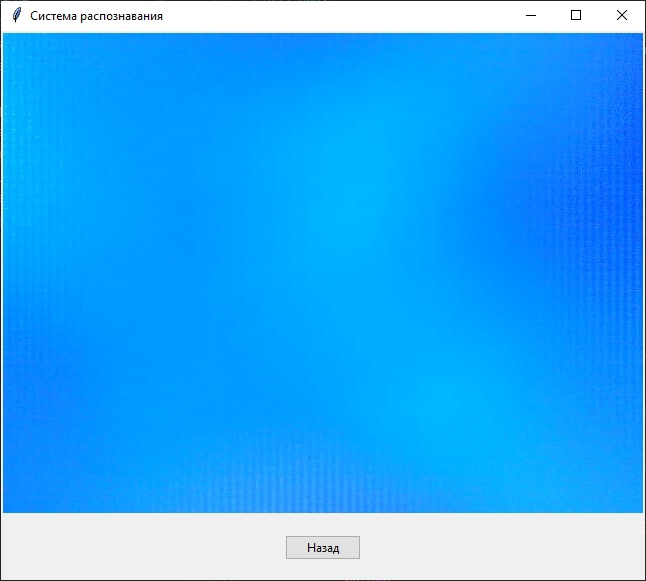
\includegraphics[width=0.7\linewidth]{images/define}
	\caption{Окно "Распознать пользователя"}
	\label{fig:define}
\end{figure}


На рисунке \ref{fig:card} представлено окно отображения ошибки при попытке использовать неподходящую карту.
\begin{figure}[H]
	\centering
	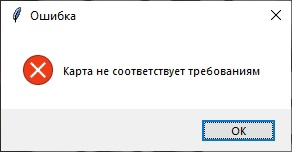
\includegraphics[width=0.65\linewidth]{images/card}
	\caption{Окно отображения ошибки "Карта не соответствует требованиям"}
	\label{fig:card}
\end{figure}


На рисунке \ref{fig:face} представлено окно отображения ошибки при попытке сканирования изображения лица, не принадлежащего владельцу карты.
\begin{figure}[H]
	\centering
	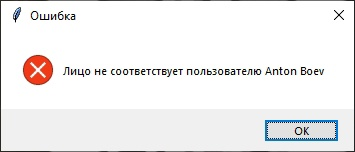
\includegraphics[width=0.65\linewidth]{images/face}
	\caption{Окно отображения ошибки "Лицо не соответствует пользователю"}
	\label{fig:face}
\end{figure}

На рисунке \ref{fig:fperror} представлено окно отображения ошибки при использовании отпечатков, не принадлежащих пользователю.
\begin{figure}[H]
	\centering
	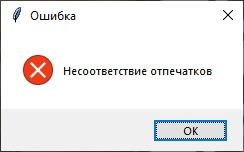
\includegraphics[width=0.6\linewidth]{images/fperror}
	\caption{Окно отображения ошибки "Несоответствие отпечатков"}
	\label{fig:fperror}
\end{figure}


\subsection{Сборка программной системы}

Программные компоненты представляют собой файлы исходных кодов программной системы.

Для сборки и компиляции программной системы использовалась библиотека Pyinstaller, позволяющая упаковать все необходимые файлы в один исполняемый файл формата .exe. Данный файл может быть запущен без предварительной установки.

Интерпретация исходных кодов на языке Python выполняется встроенным в исполняемый файл интерпретатором языка и не требует отдельной установки интерпретатора и библиотек на целевую систему.

Все программные компоненты собраны в один исполняемый файл, готовый к запуску в среде Windows.
